\section{5-state Sporadic Machines}\label{sec:sporadic}



\begin{figure}[h!]
    \centering

    % First row: 3 images
    \begin{minipage}{\textwidth}
        \centering
        \begin{subfigure}{0.3\textwidth}
            \centering
            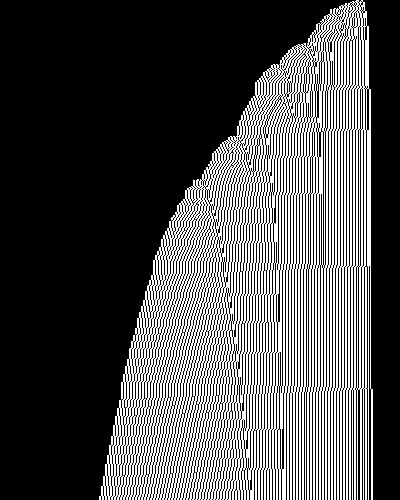
\includegraphics[width=\linewidth]{figures/sporadic-machines/sk1.png}
            \caption*{\href{https://bbchallenge.org/1RB1RD_1LC0RC_1RA1LD_0RE0LB_---1RC}{Skelet \#1}}
        \end{subfigure}
        \hfill
        \raisebox{8.5em}[0pt][0pt]{% <-- tweak this value as needed
            \begin{minipage}{0.3\textwidth}
                \centering
                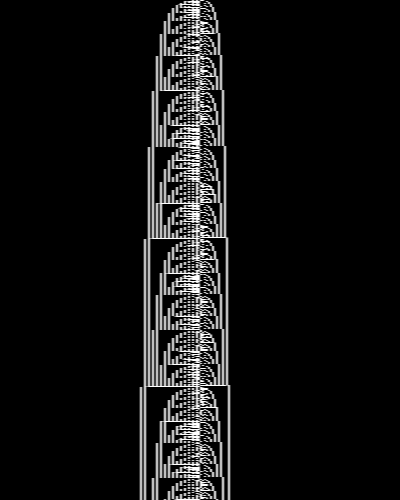
\includegraphics[width=\linewidth]{figures/sporadic-machines/sk10.png}

                \caption*{\href{https://bbchallenge.org/1RB0RA_0LC1RA_1RE1LD_1LC0LD_---0RB}{Skelet \#10}}
                {\small\emph{\href{https://bbchallenge.org/1RB0RA_0LC1RA_1RE1LD_1LC0LD_---0RB}{Double Fibonacci Counter}}}
            \end{minipage}
        }
        \hfill
        \begin{subfigure}{0.3\textwidth}
            \centering
            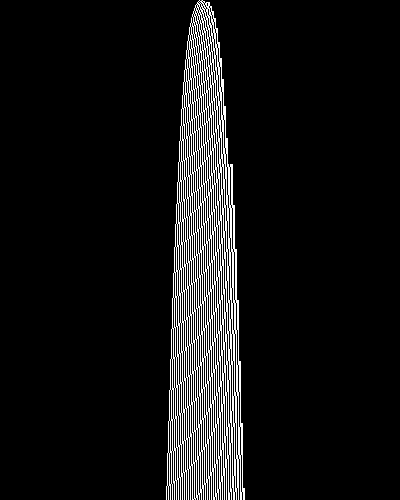
\includegraphics[width=\linewidth]{figures/sporadic-machines/sk17.png}
            \caption*{\href{https://bbchallenge.org/1RB---_0LC1RE_0LD1LC_1RA1LB_0RB0RA}{Skelet \#17}}
        \end{subfigure}
    \end{minipage}

    \vspace{2.5em}

    % Second row: Shift Overflow Counters
    \begin{tikzpicture}
        \node[draw=magenta, thick, rounded corners, inner sep=8pt] (box1) {
            \begin{minipage}{0.95\textwidth}
                \centering
                \textbf{\textcolor{magenta}{Shift Overflow Counters}}\\[0.8em]
                \begin{subfigure}{0.17\textwidth}
                    \centering
                    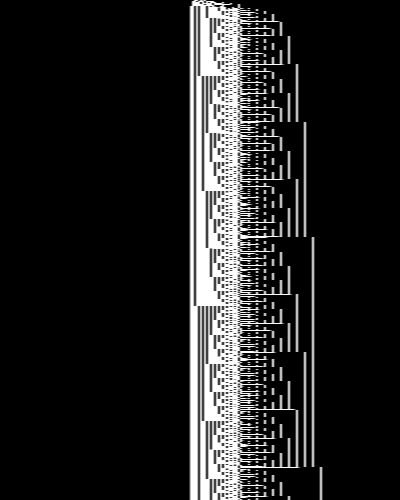
\includegraphics[width=\linewidth]{figures/sporadic-machines/soc_sk15.png}
                    \caption*{\href{https://bbchallenge.org/1RB---_1RC1LB_1LD1RE_1LB0LD_1RA0RC}{Skelet \#15}}
                \end{subfigure}
                \hfill
                \begin{subfigure}{0.17\textwidth}
                    \centering
                    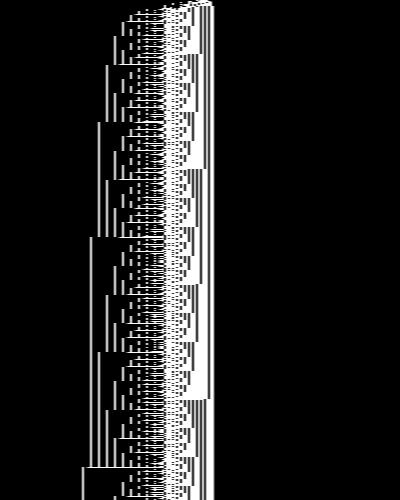
\includegraphics[width=\linewidth]{figures/sporadic-machines/soc_sk26.png}
                    \caption*{\href{https://bbchallenge.org/1RB1LD_1RC0RB_1LA1RC_1LE0LA_1LC---}{Skelet \#26}}
                \end{subfigure}
                \hfill
                \begin{subfigure}{0.17\textwidth}
                    \centering
                    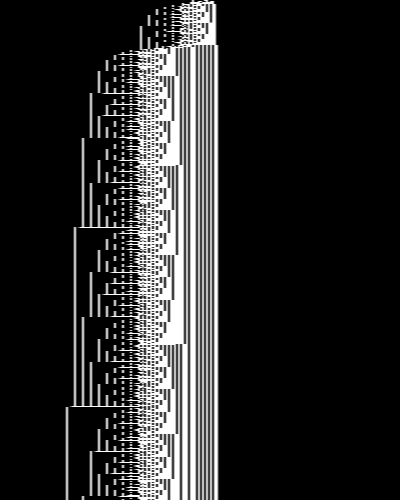
\includegraphics[width=\linewidth]{figures/sporadic-machines/soc_sk33.png}
                    \caption*{\href{https://bbchallenge.org/1RB1LC_0RC0RB_1LD0LA_1LE---_1LA1RE}{Skelet \#33}}
                \end{subfigure}
                \hfill
                \begin{subfigure}{0.17\textwidth}
                    \centering
                    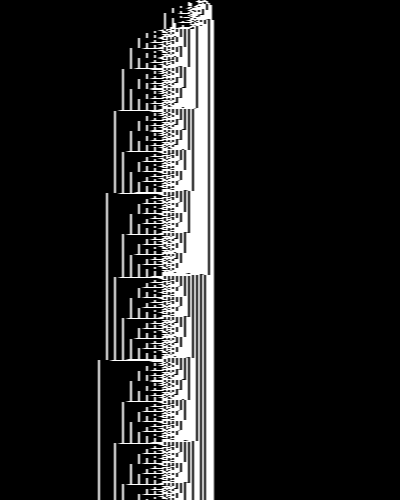
\includegraphics[width=\linewidth]{figures/sporadic-machines/soc_sk34.png}
                    \caption*{\href{https://bbchallenge.org/1RB1LC_0RC0RB_1LD0LA_1LE---_1LA1RA}{Skelet \#34}}
                \end{subfigure}
                \hfill
                \begin{subfigure}{0.17\textwidth}
                    \centering
                    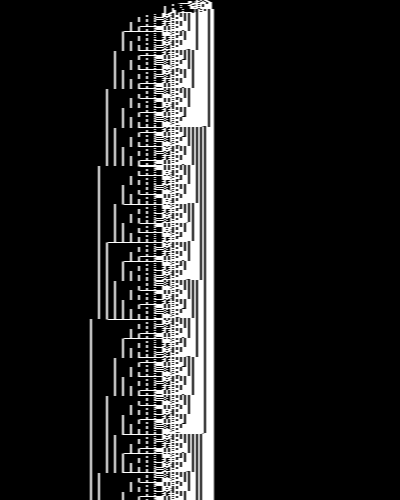
\includegraphics[width=\linewidth]{figures/sporadic-machines/soc_sk35.png}
                    \caption*{\href{https://bbchallenge.org/1RB1LC_0RC0RB_1LD0LA_1LE---_1LA0LA}{Skelet \#35}}
                \end{subfigure}
            \end{minipage}
        };
    \end{tikzpicture}

    \vspace{1.5em}

    % Third row: Finned Machines
    \begin{tikzpicture}
        \node[draw=magenta, thick, rounded corners, inner sep=8pt] (box2) {
            \begin{minipage}{0.95\textwidth}
                \centering
                \textbf{\textcolor{magenta}{Finned Machines}}\\[0.8em]
                \begin{subfigure}{0.17\textwidth}
                    \centering
                    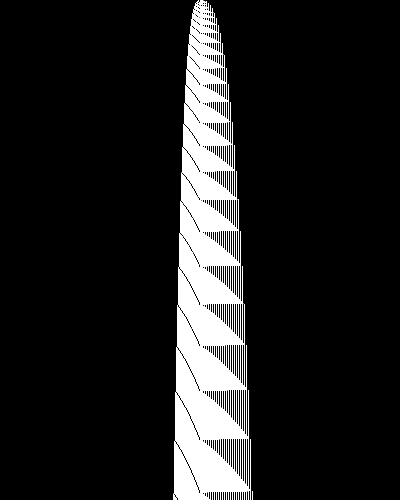
\includegraphics[width=\linewidth]{figures/sporadic-machines/finned_1.png}
                    \caption*{\href{https://bbchallenge.org/1RB0LE_1RC1RB_1RD1LC_0LE0RB_---1LA}{Finned \#1}}
                \end{subfigure}
                \hfill
                \begin{subfigure}{0.17\textwidth}
                    \centering
                    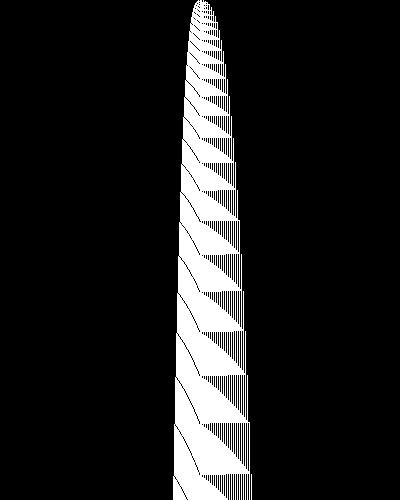
\includegraphics[width=\linewidth]{figures/sporadic-machines/finned_2.png}
                    \caption*{\href{https://bbchallenge.org/1RB1RA_1RC1LB_0LD0RA_1RA1LE_---0LD}{Finned \#2}}
                \end{subfigure}
                \hfill
                \begin{subfigure}{0.17\textwidth}
                    \centering
                    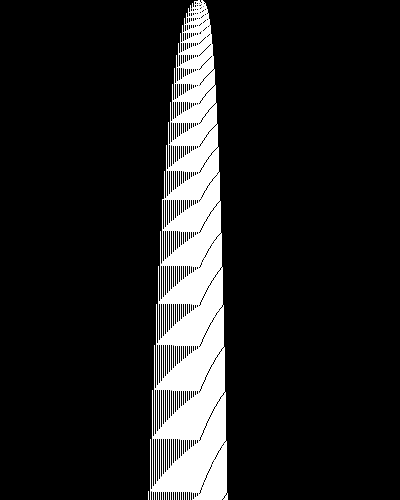
\includegraphics[width=\linewidth]{figures/sporadic-machines/finned_3.png}
                    \caption*{\href{https://bbchallenge.org/1RB1RE_1LC1RB_0RA0LD_1LB1LD_---0RA}{Finned \#3}}
                \end{subfigure}
                \hfill
                \begin{subfigure}{0.17\textwidth}
                    \centering
                    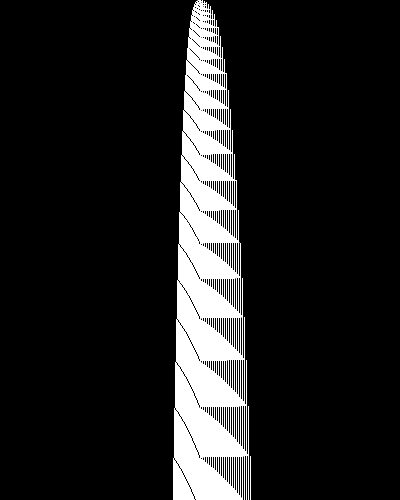
\includegraphics[width=\linewidth]{figures/sporadic-machines/finned_4.png}
                    \caption*{\href{https://bbchallenge.org/1RB1LA_0LC0RE_---1LD_1RA0LC_1RA1RE}{Finned \#4}}
                \end{subfigure}
                \hfill
                \begin{subfigure}{0.17\textwidth}
                    \centering
                    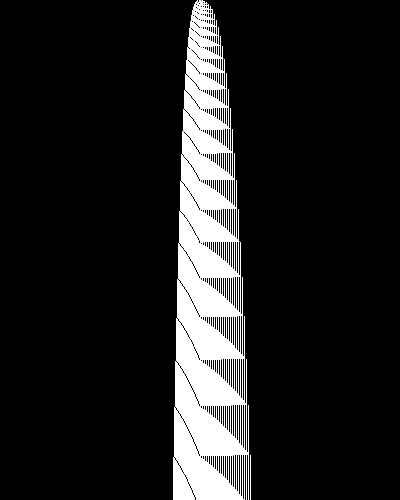
\includegraphics[width=\linewidth]{figures/sporadic-machines/finned_5.png}
                    \caption*{\href{https://bbchallenge.org/1RB1LA_0LC0RE_---1LD_1LA0LC_1RA1RE}{Finned \#5}}
                \end{subfigure}
            \end{minipage}
        };
    \end{tikzpicture}

    \caption{{\small Family picture of the 5-state Sporadic Machines (20,000-step space-time diagrams) which required individual \Coq nonhalting proofs; machine names in the Figure are clickable URLs giving the TNF-normalised transition table of each machine (see Section~\ref{sec:enum}). All Sporadic Machines were also identified by Skelet \cite{Skelet_bbfind}, either as unprovable using his \texttt{bbfind} program, or, for what we call ``Finned Machines'' marked as ``easily provable by hand'' \cite{Skelet_bbfind_list}. For better visibility, diagrams of counters (Skelet \#10 and Shift Overflow Counters) have been represented using a tape of length 200 instead of 400, giving a \textit{zoomed-in} effect.}}
    \label{fig:sporadic}
\end{figure}

Sporadic Machines are 13 nonhalting 5-state Turing machines that were not captured by deciders (Section~\ref{sec:deciders}) and required individual \Coq proofs of nonhalting; their space-time diagrams are given in Figure~\ref{fig:sporadic} where each name is a clickable URL leading to the machine's transition table and space-time diagram. Twelve of these machines, \ie all but ``Skelet \#17'' (see below), were proved nonhalting in \texttt{busycoq} \cite{busycoq}, and then integrated\footnote{For convenience, the relevant parts of \texttt{busycoq} have been added to the root of \CoqBB, at \url{https://github.com/ccz181078/Coq-BB5/tree/main/BusyCoq}. \CoqBB translates \texttt{busycoq} proofs using \href{https://github.com/ccz181078/Coq-BB5/blob/main/CoqBB5/BB5/BusyCoq_Translation.v}{\texttt{BusyCoq\_Translation.v}}.} into \CoqBB. Machine ``Skelet \#17'' was the last 5-state machine to be formally proven nonhalting in Coq, as part of \CoqBB, achieving the proof of $S(5) = \BBtheFifth$ -- a different proof also had been released as a standalone paper, \cite{xu2024skelet17fifthbusy}.

Interestingly all Sporadic Machines had been identified by Georgi Georgiev (also known as ``Skelet'', see Section~\ref{sec:intro:mainresults}) in 2003: either as part of his 43 unsolved machines\footnote{Apart from \cite{Skelet_bbfind_list}, these 43 machines are also listed here: \url{https://bbchallenge.org/skelet}.} which are named after him, \eg ``Skelet \#1'' (see Figure~\ref{fig:sporadic}), either, in the case of what we call ``Finned Machines'', marked by him as ``easily provable by hand'' \cite{Skelet_bbfind_list}. Sporadic Machines can be arranged in three buckets:
\begin{itemize}
    \item \textbf{Finned Machines.} These are five akin machines that hold 3 unary numbers on the tape (and can merge the middle one into its neighbor), vary them while maintaining a linear relation, and in the process ensure any deviation from this linear relation would be detected and cause a halt. These machines were solved by handcrafting nonhalting certificates similar in flavor to WFAR certificates (Section~\ref{sec:WFAR}). The certificates were crafted by Blanchard, translated in \Coq by mei, see \texttt{busycoq} files \texttt{Finned\{1-5\}.v}. An argument of irregularity (Section~\ref{sec:deciders-overview}) was given for machine ``Finned \#3'' \cite{irregularFinned3}. A later-developed irregular extension of RepWL (Section~\ref{sec:RepWL}) has been reported to solve these machines\footnote{\url{https://discuss.bbchallenge.org/t/bb5s-finned-machines-summary/234}}.
    \item \textbf{Shift Overflow Counters.} This family concerns Skelet's machines \href{https://bbchallenge.org/1RB---_1RC1LB_1LD1RE_1LB0LD_1RA0RC}{15}, \href{https://bbchallenge.org/1RB1LD_1RC0RB_1LA1RC_1LE0LA_1LC---}{26}, \href{https://bbchallenge.org/1RB1LC_0RC0RB_1LD0LA_1LE---_1LA1RE}{33}, \href{https://bbchallenge.org/1RB1LC_0RC0RB_1LD0LA_1LE---_1LA1RA}{34} and \href{https://bbchallenge.org/1RB1LC_0RC0RB_1LD0LA_1LE---_1LA0LA}{35}; Figure~\ref{fig:sporadic}. These machines are similar: they implement two independent binary counters, one to the left of the tape and the other to the right, and they undergo relatively complex behaviors when either counter overflows. They have been described in details by Ligocki, who first analysed them \cite{ShawnSOC}. They were then proved in \Coq by Yuen and mei as part of \texttt{busycoq}, see files \texttt{Skelet\{15,26,33,34,35\}.v} \cite{busycoq}.
    \item \textbf{\href{https://bbchallenge.org/1RB1RD_1LC0RC_1RA1LD_0RE0LB_---1RC}{Skelet \#1}, \href{https://bbchallenge.org/1RB0RA_0LC1RA_1RE1LD_1LC0LD_---0RB}{Skelet \#10}, and, \href{https://bbchallenge.org/1RB---_0LC1RE_0LD1LC_1RA1LB_0RB0RA}{Skelet \#17}.} These three machines each have unique behaviors which we detail below.
\end{itemize}

\paragraph{\href{https://bbchallenge.org/1RB1RD_1LC0RC_1RA1LD_0RE0LB_---1RC}{Skelet \#1}.} This machine is a Translated Cycler, \ie a machine that eventually repeats the same pattern translated in space (see Section~\ref{sec:loops}), but with enormous parameters: its pre-period (number of steps to wait before the pattern first appears) is about $5.42 \times 10^{51}$ and its period (number of steps taken by the repeated pattern) is $8,468,569,863$. This was discovered by means of accelerated simulation by Kropitz \cite{uniSk1} and thorough analysis by Ligocki \cite{ShawnSkelet1Before, ShawnSkelet1}. The result was confirmed correct after mei formalised it in \Coq as part of \texttt{busycoq}, see file \texttt{Skelet1.v} \cite{busycoq}. The $10^{51}$ pre-period was computed later by Huang \cite{hipparcosSk1}.



\paragraph{\href{https://bbchallenge.org/1RB0RA_0LC1RA_1RE1LD_1LC0LD_---0RB}{Skelet \#10} (Double Fibonacci Counter).} This machine implements two independent \textit{base Fibonacci} counters, one to the left of the tape and the other to the right. Counting in base Fibonacci means exploting Zeckendorf's theorem \cite{wiki:Zeckendorf's_theorem}: any natural number can be expressed as a sum of Fibonacci numbers in exactly one way, excluding using numbers immediately adjacent in the Fibonacci sequence, where the Fibonacci sequence is $F = 1,2,3,5,8,13,21,34\dots$ -- each number in the sequence is the sum of the two previous ones. For instance, $17 = 1 + 3 + 13$ and this decomposition would be represented as \texttt{100101} in big-endian binary: the $i^\text{th}$ bit from the right is $1$ if we use $F_i$ in the sum. Each of the two counters of Skelet \#10 enumerate natural numbers in base Fibonacci, using slightly different encodings and the machine halts iff the counters ever get out of sync -- which, does not happen. The machine was analysed independently by Briggs and Ligocki \cite{DanBriggs,ShawnSkelet10} and Ligocki's proof \cite{ShawnSkelet10} was formalised in \Coq by mei as part of \texttt{busycoq}, see file \texttt{Skelet10.v} \cite{busycoq}. Skelet \#10 is the only known \textit{double} 5-state Fibonnaci counter, but there are several known \textit{single} Fibonnaci counters, such as \href{https://bbchallenge.org/1RB0RA_0LC1RA_1LD0LC_1RE1LC_---0RB}{\texttt{1RB0RA\_0LC1RA\_1LD0LC\_1RE1LC\_---0RB}}, solved by \CoqBB's NGramCPS (Section~\ref{sec:n-gramCPS}).

% Fibonacci notation is a binary notation where the $n^\text{th}$ bit, instead of representing $2^n$ as in standard binary, represents $F_{n+2}$ where $F = 0,1,1,2,3,5,8,13,21,34\dots$ is the Fibonacci sequence (each number is the sum of the previous two). For instance, in big-endian notation, \texttt{100101} represents $F_{5+2} + F_{2+2} + F_{0+2} = 13 + 3 + 1 = 17$.

\paragraph{\href{https://bbchallenge.org/1RB---_0LC1RE_0LD1LC_1RA1LB_0RB0RA}{Skelet \#17}.} \textit{The final boss.} This machine manages a list of integers $n_1, \dots, n_k \in \mathbb{N}$ represented in unary on the tape using encoding: $(\texttt{10})^{n_1} (\texttt{10})^{n_2} \dots (\texttt{10})^{n_k}$. The list can only increase and undergoes a set of complex transformations related to Gray code, and, the machine halts iff $n_1 = n_2 = 0$ and $n_3,\, \dots,\, n_k$ are all even. Showing that this never happens, \ie the machine does not halt, was first drafted by savask \cite{savaskSk17}, made into a standalone paper by Xu \cite{xu2024skelet17fifthbusy} and, finally, using a different argument, proved in \Coq by mxdys as part of \CoqBB. Skelet \#17 was the last 5-state machine to be solved in \Coq.